\subsection{Open Agriculture Initiative - Personal Food Computer}

% Project Homepage: https://www.media.mit.edu/groups/open-agriculture-openag/overview/
% Design Repositories: https://github.com/OpenAgricultureFoundation
% PFC White Paper: PDF in Discord
    % Citation: \cite{mit-openag}
% OpenAG White Paper: PDF in Discord
    % Citation: \cite{mit-pfc}

% Half-decent summary: https://www.notion.so/Open-Agriculture-Initiative-OpenAG-cfa5031e2b244093a37158fe1a99ec12

\subsubsection{Overview}

The Open Agriculture Initiative (OpenAG) was a project launched by the MIT Media Lab with the goal to "Build open resources to enable a global community to accelerate digital agricultural innovation" \cite{mit-openag}.

One of their primary developments was an open-source controlled-environment agriculture micro-greenhouse, the Personal Food Computer (PFC) \cite{mit-pfc}. The PFC controls all environmental growing parameters and collects data during the growth cycle.
Data can be collected by users and shared between members of the open-source community. This allows for the creation of reproducible "climate recipes" where other devices with similar abilities can reliably generate the same environment and (ideally) attain the same plant growth results.

\begin{figure}[h]
    \centering
    \begin{subfigure}[b]{0.08\textwidth}
        \hfill
    \end{subfigure}
    \begin{subfigure}[b]{0.40\textwidth}
        \centering
        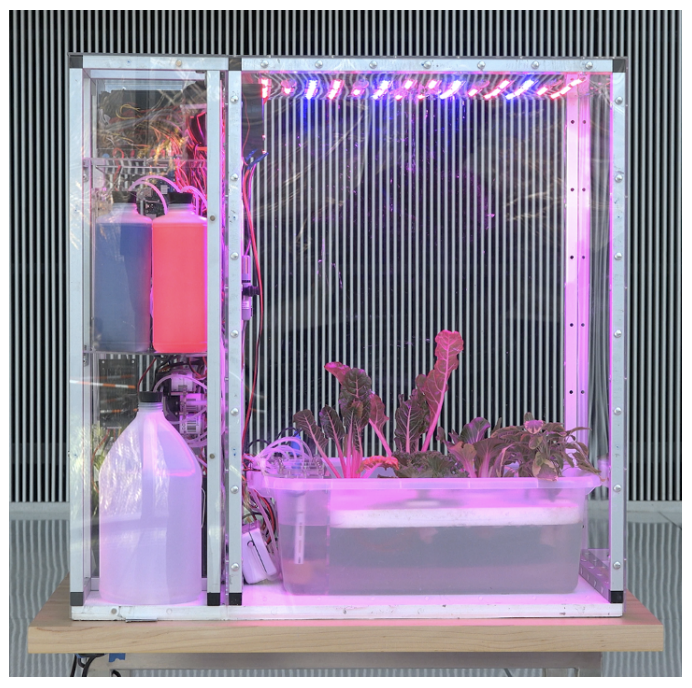
\includegraphics[width=\textwidth]{../assets/pfc-built.png}
        \caption{Assembled PFC v1}
        \label{fig:pfc-built}
    \end{subfigure}
    \hfill
    \begin{subfigure}[b]{0.26\textwidth}
        \centering
        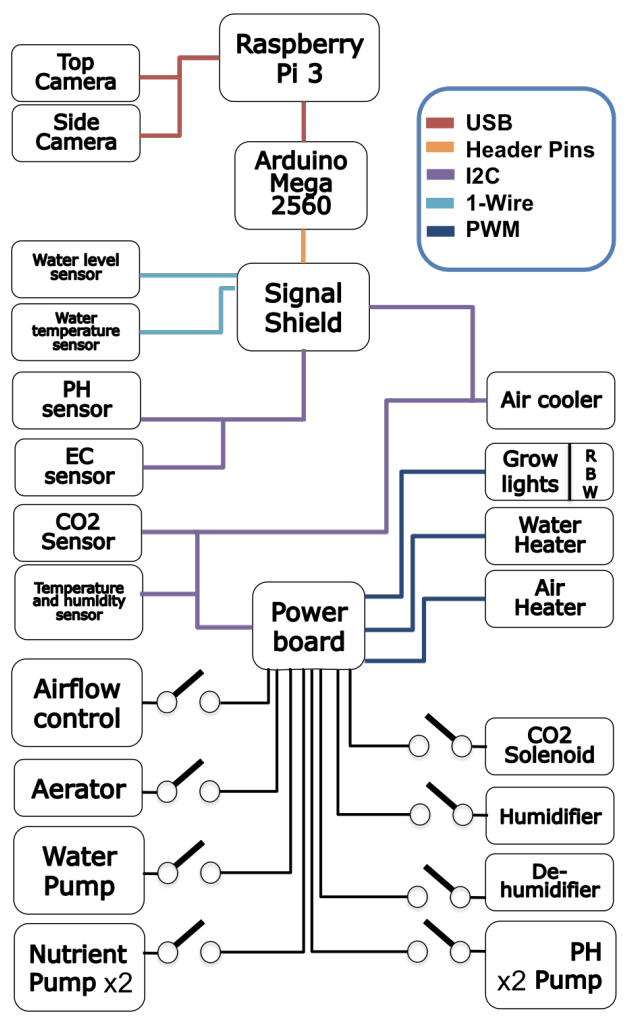
\includegraphics[width=\textwidth]{../assets/pfc-components.png}
        \caption{PFC component diagram}
        \label{fig:pfc-components}
    \end{subfigure}
    \begin{subfigure}[b]{0.10\textwidth}
        \hfill
    \end{subfigure}
    \caption{Personal Food Computer v1 \cite{mit-pfc}}
    \label{fig:pfc}
\end{figure}

\subsubsection{Analysis}

One of the design's major flaws is in its implementation. Despite the claim that the PFC focusses on viable environment generation (Scope \ref{sc:3a}-\ref{sc:3c}) and continuity and range of environment conditions (Scope \ref{sc:5}) \cite{mit-basil}, in practice, it failed to produce food outputs (Requirement \ref{r:1}) \cite{mit-wfp}.
In addition, the PFC utilizes Deep Water Culture (DWC) hydroponics \cite{mit-pfc}, as opposed to aeroponics, resulting in a lowered water efficiency (Objective \ref{ll:efficiency_water}) and decreased control over water conditions (Objective \ref{ll:control_nutrientsolution}).

However, the array of sensors and actuators included in the design (See \ref{fig:pfc-components}), as well as the principle of plant phenomenology optimization \cite{mit-openag}, is informative in meeting Requirement \ref{r:3} and their attempts can serve as a basis for understanding Scope \ref{sc:3} and \ref{sc:5}.

\subsubsection{Assessment}

\textbf{Objectives Considered}: \ref{ll:output_variety}, \ref{ll:output_palatability} (via \ref{sc:5}), \ref{ll:control_airtemp}. \ref{ll:control_airhum}, \ref{ll:control_light}, \ref{ll:control_aircirculation}, \ref{ll:control_nutrientsolution}, \ref{ll:automation}

\textbf{Objectives Not Considered}: \ref{ll:output_energy}, \ref{ll:insulateisolate}, \ref{ll:germinationsuccess}, \ref{ll:efficiency_energy}, \ref{ll:efficiency_water}, \ref{ll:time_germination}, \ref{ll:time_growth}, \ref{ll:time_harvest}, \ref{ll:crosscontamination}

\begin{figure}[h]
    \centering
    \begin{tabular}{|l|l|c|}
        \hline
        \textbf{Metric}                     & \textbf{Value}    & \textbf{Met?}         \\ \hline
        \mref{m:palatability}               & N/A (Presumed Y)  & \cellcolor{red} N     \\ \hline
        \mref{m:airtemp_range}              & N/A (Presumed Y)  & \cellcolor{red} N     \\ \hline % TODO: Source?
        \mref{m:airhum_range}               & N/A (Presumed Y)  & \cellcolor{red} N     \\ \hline % TODO: Source?
        \mref{m:co2_range}                  & N/A (Presumed N)  & \cellcolor{red} N     \\ \hline
        \mref{m:light_waverange}            & 448-710nm         & \cellcolor{red} N     \\ \hline % TODO: Source? Disinfection?
        \mref{m:light_parmatch}             & 100\%             & \cellcolor{green} Y   \\ \hline % TODO: Source?
        \mref{m:lightintensity_range}       & N/A (Presumed Y)  & \cellcolor{red} N     \\ \hline % TODO: Source?
        \mref{m:circulation_range}          & N/A (Presumed Y)  & \cellcolor{red} N     \\ \hline
        \mref{m:solutionrate_range}         & N/A (Presumed Y)  & \cellcolor{red} N     \\ \hline % TODO: Source?
        \mref{m:solutiontemp_range}         & N/A (Presumed Y)  & \cellcolor{red} N     \\ \hline % TODO: Source?
        \mref{m:nutrient_range}             & N/A (Presumed Y)  & \cellcolor{red} N     \\ \hline % TODO: Source?
        \mref{m:time_maintenance}           & N/A (Presumed Y)  & \cellcolor{red} N     \\ \hline
        \mref{m:efficiency_water}           & N/A (Presumed N)  & \cellcolor{red} N     \\ \hline
        \mref{m:water_initial}              & N/A (Presumed Y)  & \cellcolor{red} N     \\ \hline
        \mref{m:hazard_chemical_materials}  & Y                 & \cellcolor{green} Y   \\ \hline
        \mref{m:hazard_chemical_inputs}     & Y                 & \cellcolor{green} Y   \\ \hline
        \mref{m:hazard_chemical_byproducts} & N                 & \cellcolor{red} N     \\ \hline
        \mref{m:hazard_chemical_outputs}    & N                 & \cellcolor{red} N     \\ \hline
        \mref{m:hazard_chemical_process}    & Y                 & \cellcolor{green} Y   \\ \hline
        \mref{m:hazard_pathogen_materials}  & N                 & \cellcolor{red} N     \\ \hline
        \mref{m:hazard_pathogen_inputs}     & N                 & \cellcolor{red} N     \\ \hline
        \mref{m:hazard_pathogen_byproducts} & N                 & \cellcolor{red} N     \\ \hline
        \mref{m:hazard_pathogen_outputs}    & N                 & \cellcolor{red} N     \\ \hline
        \mref{m:hazard_pathogen_process}    & N                 & \cellcolor{red} N     \\ \hline
        \mref{m:shelflife_output}           & N/A (Presumed N)  & \cellcolor{red} N     \\ \hline
        \mref{m:dimensions}                 & Y                 & \cellcolor{green} Y   \\ \hline % TODO: Dimensions?
        \mref{m:volume}                     & Y                 & \cellcolor{green} Y   \\ \hline % TODO: Volume?
        \mref{m:power}                      & N/A (Presumed Y)  & \cellcolor{red} N     \\ \hline
    \end{tabular}
    \caption{Constraint Assessment: 6/40 (15\%) met.\\Metrics without values omitted for concision.}
\end{figure}